% Results section, included from report.tex. All tables are generated by
% scripts/make_report_tables.py from output/scenarios/scenario-results.json.

\subsubsection*{A. Service acceptance}

Table~\ref{tab:acc} and Figure~\ref{fig:acc} give hold-out acceptance for every
scenario. The main scenarios are heavy load: offered demand at 90\%, 100\% and
110\% of the network's compute capacity. Updated FPPVS reaches the 70\% target in
all six main scenarios. Its mean acceptance ranges from \fppvsMinAcc\%
(\fppvsWorstScenario) to \fppvsMaxAcc\%, with an average of \fppvsMeanAcc\%. The
lowest value in any single seed was \fppvsLowestRun\%, so the target also holds
run by run, not only on average.

\begin{table}[H]
\centering\footnotesize
\setlength{\tabcolsep}{4pt}
\caption{Hold-out service acceptance (\%), mean $\pm$ standard deviation over
\numSeeds{} seeds. Best value per row in bold.}
\label{tab:acc}
\begin{tabular}{lccccc}
\toprule
Scenario (topology, load) & Updated (ours) & Original FPPVS & 2022 adaptation & Greedy & Random \\
\midrule
Backbone 0.9 & \textbf{91.0 $\pm$ 3.6} & 45.0 $\pm$ 4.8 & 47.8 $\pm$ 7.6 & 58.7 $\pm$ 4.4 & 57.4 $\pm$ 4.0 \\
Backbone 1 & \textbf{86.4 $\pm$ 3.7} & 43.6 $\pm$ 5.1 & 44.5 $\pm$ 6.5 & 53.4 $\pm$ 5.1 & 55.3 $\pm$ 3.4 \\
Backbone 1.1 & \textbf{80.8 $\pm$ 3.8} & 40.9 $\pm$ 5.3 & 43.0 $\pm$ 10.4 & 51.9 $\pm$ 4.9 & 52.9 $\pm$ 3.3 \\
Metro 0.9 & \textbf{86.1 $\pm$ 2.9} & 50.2 $\pm$ 5.8 & 53.1 $\pm$ 9.3 & 56.3 $\pm$ 3.1 & 56.6 $\pm$ 3.0 \\
Metro 1 & \textbf{81.3 $\pm$ 3.5} & 49.7 $\pm$ 4.5 & 49.4 $\pm$ 9.7 & 51.8 $\pm$ 3.6 & 52.6 $\pm$ 3.0 \\
Metro 1.1 & \textbf{76.6 $\pm$ 2.5} & 47.2 $\pm$ 5.0 & 50.1 $\pm$ 5.2 & 48.8 $\pm$ 1.9 & 50.9 $\pm$ 3.1 \\
\midrule \multicolumn{6}{l}{\emph{Other load levels (light load and overload)}} \\
Backbone 0.5 & \textbf{99.6 $\pm$ 0.4} & 58.1 $\pm$ 4.1 & 68.1 $\pm$ 5.4 & 72.1 $\pm$ 5.8 & 73.2 $\pm$ 4.5 \\
Backbone 1.25 & \textbf{75.2 $\pm$ 2.9} & 38.7 $\pm$ 3.9 & 41.1 $\pm$ 3.0 & 49.3 $\pm$ 3.8 & 50.9 $\pm$ 2.7 \\
Backbone 1.5 & \textbf{65.2 $\pm$ 3.3} & 35.0 $\pm$ 4.2 & 38.4 $\pm$ 4.3 & 43.4 $\pm$ 4.1 & 44.2 $\pm$ 2.1 \\
Metro 0.5 & \textbf{99.0 $\pm$ 0.8} & 64.6 $\pm$ 10.2 & 74.0 $\pm$ 9.7 & 71.4 $\pm$ 3.0 & 72.1 $\pm$ 2.9 \\
Metro 1.25 & \textbf{69.2 $\pm$ 4.2} & 44.0 $\pm$ 2.9 & 40.5 $\pm$ 7.8 & 47.2 $\pm$ 2.1 & 46.9 $\pm$ 2.3 \\
Metro 1.5 & \textbf{60.6 $\pm$ 1.9} & 36.7 $\pm$ 5.0 & 42.2 $\pm$ 3.9 & 42.2 $\pm$ 2.7 & 43.1 $\pm$ 1.3 \\
\bottomrule
\end{tabular}
\end{table}

\begin{figure}[H]
\centering
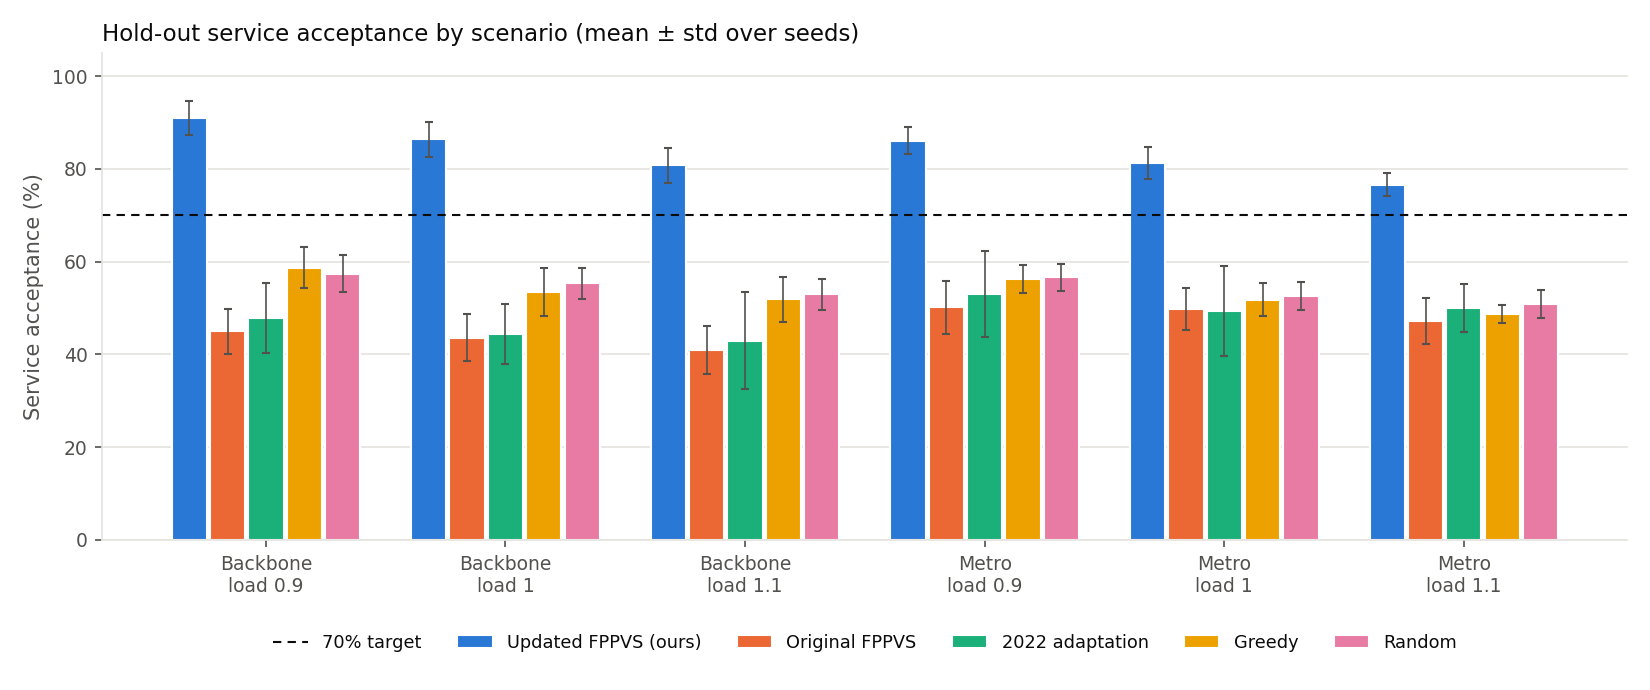
\includegraphics[width=\linewidth]{scenario-acceptance.png}
\caption{Hold-out acceptance in the six main scenarios. Error bars show one
standard deviation over seeds; the dashed line is the 70\% target.}
\label{fig:acc}
\end{figure}

\needspace{5\baselineskip}
\paragraph{Observations.}
\begin{itemize}
  \item Updated FPPVS is the best method in every scenario. At full load
  ($\rho=1$) it accepts 86.4\% on Backbone and 81.3\% on Metro, and at 10\%
  overload ($\rho=1.1$) still 80.8\% and 76.6\%.
  \item The original FPPVS reaches \origMinAcc--\origMaxAcc\% in the main
  scenarios (mean \origMeanAcc\%), and the 2022 adaptation reaches
  \zhangMinAcc--\zhangMaxAcc\% (mean \zhangMeanAcc\%). Updated FPPVS is
  \origGainMean{} points above the original and \zhangGainMean{} points above
  the 2022 adaptation on average.
  \item Both learning baselines score below greedy and random in most
  scenarios. The reason is how infeasible choices are handled. Greedy and random
  run with our feasibility mask, so they never pick a DC that is already known to
  break bandwidth or latency. The original FPPVS and the 2022 adaptation check
  only compute while placing, as their methods describe, and find bandwidth and
  latency violations only when the whole chain is done (see Part E).
  \item The 2022 adaptation is the least stable method: its standard deviation
  across seeds reaches 10 points (Backbone, $\rho=1.1$). One reward value per
  episode (LTCR) gives the agent a weak learning signal.
  \item Greedy and random accept 49--59\%. They spread VNFs over many DCs, so
  each request uses about twice as much link bandwidth as updated FPPVS
  (Section~C), and links run out first.
  \item Metro is harder than Backbone at the same load. It has fewer DCs and
  fewer links, so there are fewer alternative paths when a link fills up.
\end{itemize}

\begin{figure}[H]
\centering
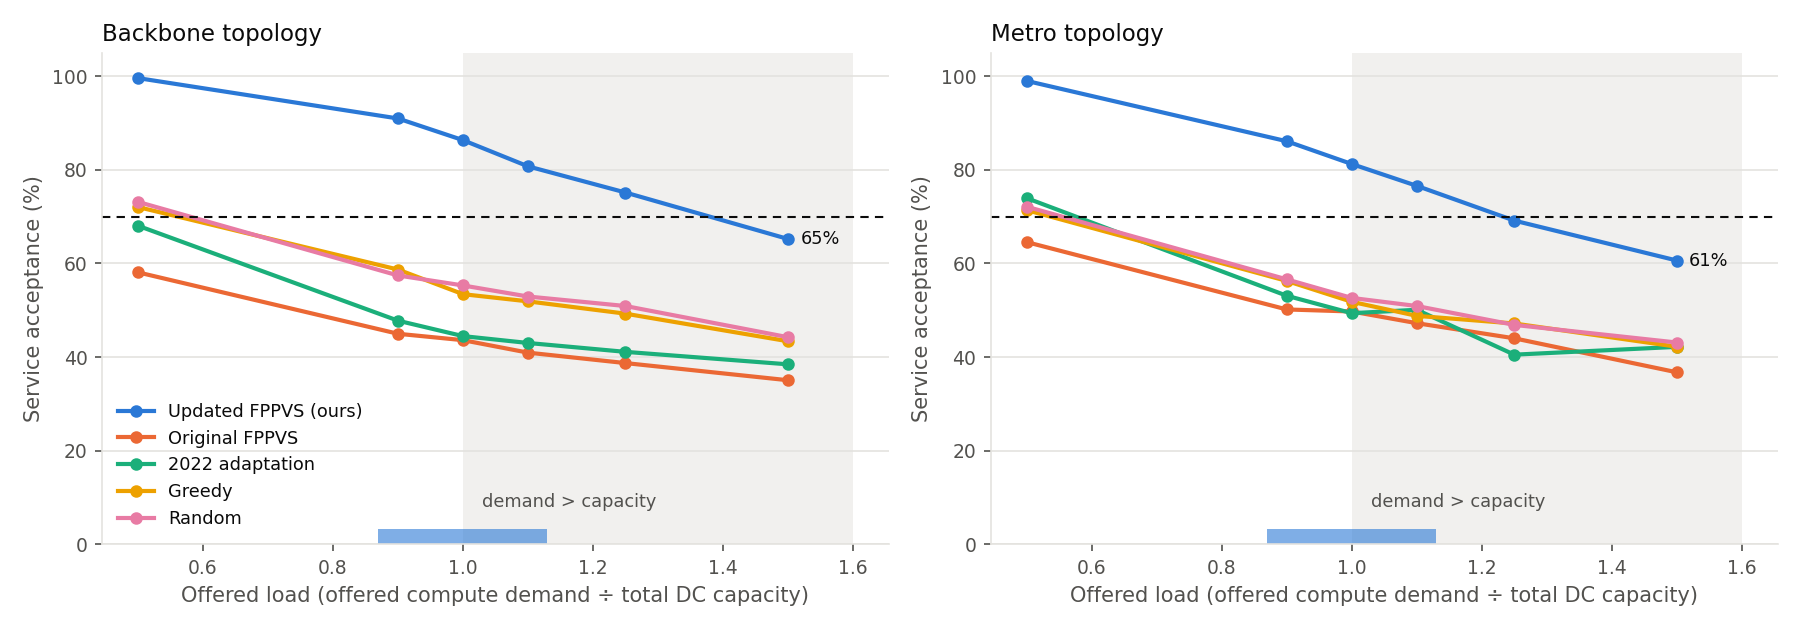
\includegraphics[width=\linewidth]{load-sweep.png}
\caption{Acceptance against offered load, from light load (0.5) to 50\%
overload (1.5). The shaded area is where the average offered compute is larger
than the total compute of the network; the blue mark on the x-axis shows the
main scenarios.}
\label{fig:sweep}
\end{figure}

\paragraph{Load sweep.} Figure~\ref{fig:sweep} shows the full range of loads. At
light load ($\rho=0.5$) updated FPPVS accepts 99.6\% (Backbone) and 99.0\%
(Metro). This is expected: with the network only half full, almost every request
fits as long as chains are kept compact. That is why we use heavier loads as the
main scenarios. As load rises, acceptance falls smoothly: 75.2\% and 69.2\% at
$\rho=1.25$, and 65.2\% and 60.6\% at $\rho=1.5$. All other methods stay at or
below 51\% in this overload region. Below 70\% is unavoidable there: at
$\rho=1.5$ only about two thirds of the offered compute can fit in the network at
any time, whatever the placement policy.

\subsubsection*{B. Ablation study}

\begin{table}[H]
\centering\small
\caption{Ablation: hold-out acceptance (\%) of updated FPPVS with one part
switched off at a time.}
\label{tab:ablation}
\begin{tabular}{lcccccc}
\toprule
Scenario & Full & w/o sharing & w/o fairness & 1 agent & w/o retry & Prior only \\
\midrule
Backbone 0.9 & 91.0 $\pm$ 3.6 & 78.7 $\pm$ 3.7 & 91.4 $\pm$ 3.2 & 90.9 $\pm$ 2.0 & 90.9 $\pm$ 2.8 & 91.9 $\pm$ 3.1 \\
Backbone 1 & 86.4 $\pm$ 3.7 & 73.8 $\pm$ 3.1 & 85.6 $\pm$ 3.9 & 86.0 $\pm$ 3.4 & 85.4 $\pm$ 3.1 & 86.3 $\pm$ 2.8 \\
Backbone 1.1 & 80.8 $\pm$ 3.8 & 68.2 $\pm$ 2.7 & 80.4 $\pm$ 4.1 & 81.2 $\pm$ 3.2 & 80.2 $\pm$ 3.5 & 80.9 $\pm$ 3.0 \\
Metro 0.9 & 86.1 $\pm$ 2.9 & 76.1 $\pm$ 2.1 & 86.8 $\pm$ 3.1 & 86.2 $\pm$ 3.0 & 86.0 $\pm$ 2.9 & 86.1 $\pm$ 3.1 \\
Metro 1 & 81.3 $\pm$ 3.5 & 70.6 $\pm$ 3.2 & 81.1 $\pm$ 2.9 & 81.0 $\pm$ 3.2 & 81.9 $\pm$ 4.0 & 81.7 $\pm$ 3.2 \\
Metro 1.1 & 76.6 $\pm$ 2.5 & 64.5 $\pm$ 2.8 & 75.7 $\pm$ 3.8 & 75.9 $\pm$ 3.8 & 76.4 $\pm$ 3.7 & 76.4 $\pm$ 2.9 \\
\bottomrule
\end{tabular}
\end{table}

Table~\ref{tab:ablation} switches off one part of updated FPPVS at a time.
\begin{itemize}
  \item \textbf{VNF sharing matters most.} Without it, acceptance falls by 10--13
  points in every main scenario (for example 86.4\% to 73.8\% on Backbone at
  $\rho=1$). Every VNF then pays its own instance overhead, so the DCs fill up
  sooner.
  \item \textbf{Fairness bonus, single vs.\ federated training and retries}
  change acceptance by about one point or less, which is within the
  seed-to-seed spread. Fairness is meant to balance throughput between flows, not
  to raise acceptance, so this is expected. Retries help only in the rare case
  where the first placement hits a dead end.
  \item \textbf{The learned network adds little over its prior.} ``Prior only''
  uses the same mask, prior and retries with no neural network, and it is within
  about one point of the full method everywhere. We report this openly: in our
  experiments the gains come mainly from the problem modifications (mask, sharing
  model, prior), not from the reinforcement learning itself. One reason is
  limitation L6: each episode covers only one request, so the agent sees little
  of the long-term effect of its choices.
\end{itemize}

\subsubsection*{C. Resource usage}

Figure~\ref{fig:res} and Table~\ref{tab:res} show the resources each method holds
for the services it runs. Table~\ref{tab:savings} summarises the difference
between updated FPPVS and each other method, averaged over the six main
scenarios.

\begin{figure}[H]
\centering
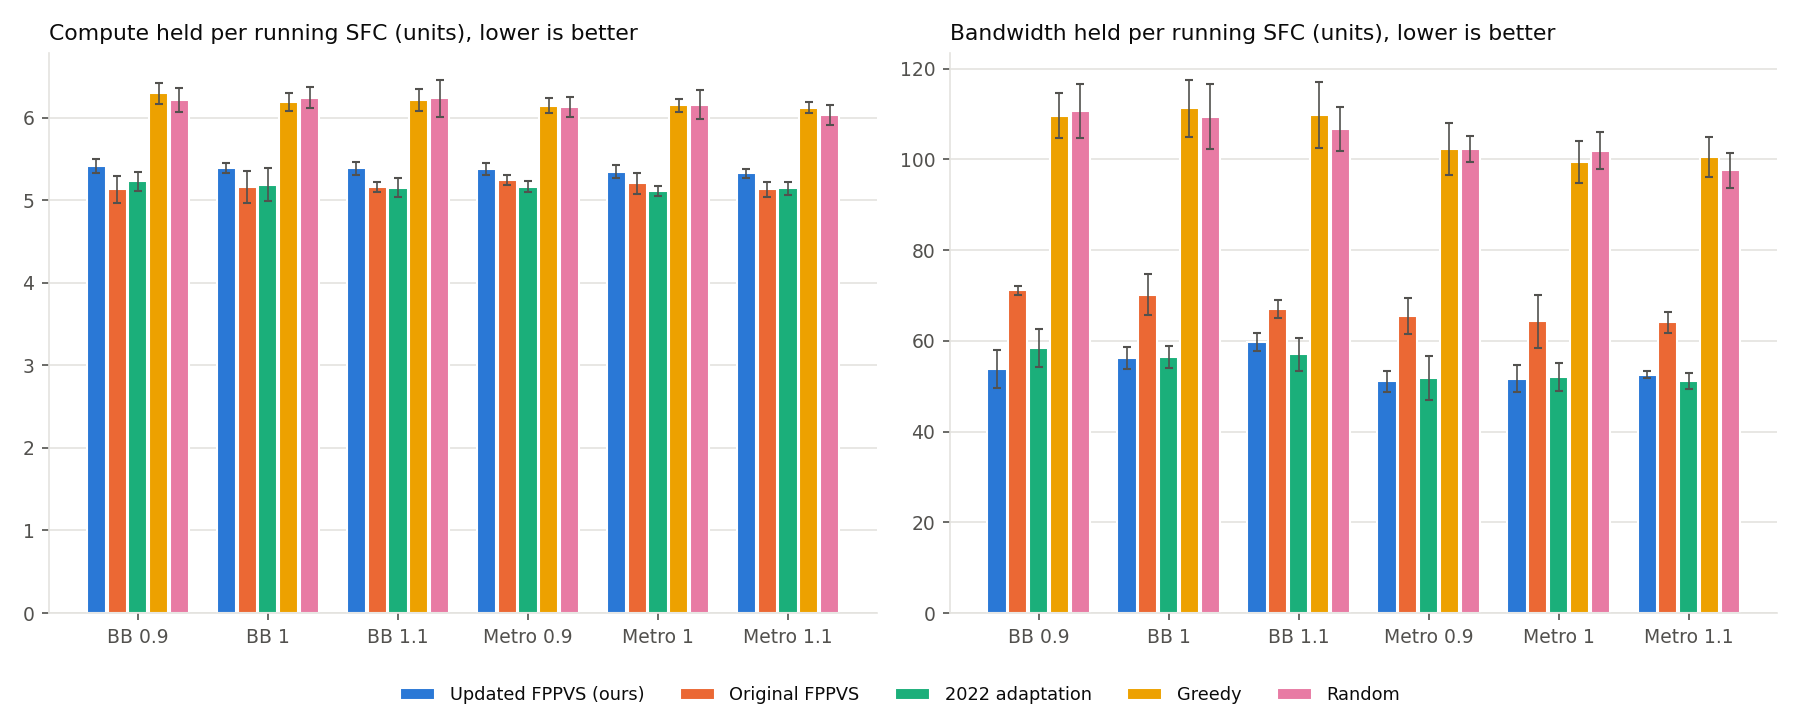
\includegraphics[width=\linewidth]{scenario-resources.png}
\caption{Compute (left) and bandwidth (right) held per running SFC, averaged over
time. Lower means each service costs less to keep running.}
\label{fig:res}
\end{figure}

\begin{table}[H]
\centering\small
\caption{Average reduction in resource use achieved by updated FPPVS over each
method (main scenarios; positive means updated FPPVS uses less, negative means
it uses more).}
\label{tab:savings}
\begin{tabular}{lcccc}
\toprule
Reduction vs. & Compute & Bandwidth & BW$\cdot$time & Instances \\
 & per SFC & per SFC & per accepted & per accepted \\
\midrule
Original FPPVS & -3.9\% & +19.2\% & +18.9\% & +13.6\% \\
2022 adaptation & -4.0\% & +0.5\% & +2.1\% & +13.7\% \\
Greedy & +13.1\% & +48.7\% & +49.4\% & +91.8\% \\
Random & +12.9\% & +48.3\% & +48.6\% & +91.8\% \\
\bottomrule
\end{tabular}
\end{table}

\begin{table}[H]
\centering\scriptsize
\setlength{\tabcolsep}{4pt}
\caption{Resource use and latency per scenario (mean over seeds; best per
column within a scenario in bold). ``Per acc.'' means per accepted SFC.}
\label{tab:res}
\begin{tabular}{llcccccc}
\toprule
Scenario & Method & Compute & Bandwidth & Compute$\cdot$time & BW$\cdot$time & Instances & Latency \\
 & & per SFC & per SFC & per acc. ($10^3$) & per acc. ($10^3$) & per acc. & (ms) \\
\midrule
Backbone 0.9 & Updated (ours) & 5.42 & \textbf{53.8} & 5.43 & \textbf{54.0} & \textbf{0.57} & \textbf{46.5} \\
 & Original FPPVS & \textbf{5.14} & 71.2 & \textbf{5.08} & 70.5 & 0.59 & 65.6 \\
 & 2022 adaptation & 5.23 & 58.4 & 5.37 & 60.0 & 0.59 & 66.2 \\
 & Greedy & 6.29 & 109.6 & 6.31 & 109.8 & 6.66 & 107.8 \\
 & Random & 6.22 & 110.7 & 6.40 & 114.0 & 6.57 & 108.8 \\
\midrule
Backbone 1 & Updated (ours) & 5.39 & \textbf{56.2} & 5.42 & \textbf{56.5} & \textbf{0.53} & \textbf{50.0} \\
 & Original FPPVS & \textbf{5.16} & 70.2 & \textbf{5.20} & 70.8 & 0.59 & 64.2 \\
 & 2022 adaptation & 5.19 & 56.5 & 5.28 & 57.4 & 0.61 & 67.2 \\
 & Greedy & 6.19 & 111.2 & 6.40 & 115.1 & 6.58 & 107.7 \\
 & Random & 6.24 & 109.4 & 6.27 & 110.1 & 6.58 & 108.1 \\
\midrule
Backbone 1.1 & Updated (ours) & 5.39 & 59.6 & 5.40 & 59.9 & \textbf{0.52} & \textbf{53.2} \\
 & Original FPPVS & 5.16 & 66.9 & \textbf{5.17} & 67.1 & 0.63 & 63.6 \\
 & 2022 adaptation & \textbf{5.15} & \textbf{57.0} & 5.26 & \textbf{58.2} & 0.63 & 70.2 \\
 & Greedy & 6.21 & 109.9 & 6.30 & 111.5 & 6.59 & 107.4 \\
 & Random & 6.23 & 106.7 & 6.24 & 107.0 & 6.56 & 108.8 \\
\midrule
Metro 0.9 & Updated (ours) & 5.38 & \textbf{51.1} & 5.50 & \textbf{52.3} & \textbf{0.55} & \textbf{45.8} \\
 & Original FPPVS & 5.24 & 65.5 & 5.42 & 67.8 & 0.64 & 62.0 \\
 & 2022 adaptation & \textbf{5.17} & 51.8 & \textbf{5.28} & 53.1 & 0.67 & 65.5 \\
 & Greedy & 6.15 & 102.2 & 6.27 & 104.6 & 6.56 & 105.2 \\
 & Random & 6.13 & 102.2 & 6.22 & 103.9 & 6.47 & 105.9 \\
\midrule
Metro 1 & Updated (ours) & 5.35 & \textbf{51.6} & 5.44 & \textbf{52.5} & \textbf{0.55} & \textbf{48.6} \\
 & Original FPPVS & 5.21 & 64.3 & \textbf{5.28} & 65.4 & 0.67 & 62.2 \\
 & 2022 adaptation & \textbf{5.11} & 52.0 & 5.35 & 54.4 & 0.62 & 67.2 \\
 & Greedy & 6.15 & 99.4 & 6.46 & 104.4 & 6.53 & 104.1 \\
 & Random & 6.16 & 101.9 & 6.38 & 105.6 & 6.51 & 105.2 \\
\midrule
Metro 1.1 & Updated (ours) & 5.33 & 52.6 & 5.43 & 53.6 & \textbf{0.51} & \textbf{50.2} \\
 & Original FPPVS & \textbf{5.13} & 64.1 & \textbf{5.12} & 64.0 & 0.62 & 62.4 \\
 & 2022 adaptation & 5.14 & \textbf{51.2} & 5.32 & \textbf{53.0} & 0.63 & 65.2 \\
 & Greedy & 6.12 & 100.5 & 6.34 & 104.1 & 6.52 & 105.0 \\
 & Random & 6.03 & 97.6 & 6.14 & 99.4 & 6.41 & 104.0 \\
\bottomrule
\end{tabular}
\end{table}

\needspace{5\baselineskip}
\paragraph{Observations.}
\begin{itemize}
  \item \textbf{Bandwidth.} Updated FPPVS holds about half the link bandwidth per
  running SFC of greedy and random (48--49\% less) and 19\% less than the
  original FPPVS. Against the 2022 adaptation it is about even: 0.5\% less on
  average, lower at $\rho=0.9$ and $\rho=1.0$, and slightly higher at
  $\rho=1.1$. Keep in mind that updated FPPVS carries 1.5--1.9 times as many
  requests as the 2022 adaptation at the same time, including harder ones that
  the other method rejects.
  \item \textbf{Instances.} Updated FPPVS starts 0.51--0.57 new VNF instances per
  accepted request, about 14\% fewer than the original FPPVS and the 2022
  adaptation and about 92\% fewer than greedy and random (about 6.6, one per VNF,
  since they do not share).
  \item \textbf{Compute.} Against greedy and random it needs about 13\% less
  compute per service, because it shares instances. Against the original FPPVS
  and the 2022 adaptation it uses about 4\% more compute per service. Those two
  methods accept far fewer requests, most likely the easier ones, so their
  per-request averages come from an easier set. The difference is small next to
  the 36--38 points of extra acceptance.
  \item \textbf{Latency.} Mean latency of accepted requests is 46--53\,ms for
  updated FPPVS, 62--70\,ms for the original FPPVS and the 2022 adaptation, and
  104--109\,ms for greedy and random. All are below the 100--150\,ms limits.
  The 2022 adaptation places the chain strictly in sequence (no parallel
  branches), so every monitor adds to the critical path.
  \item \textbf{Decision time.} Updated FPPVS needs 9--13\,ms per request,
  including the CNN forward pass and occasional retries. Greedy and random take
  2--3\,ms. Training one updated FPPVS model with 2000 episodes takes about
  \trainSeconds\,s on the CPU.
\end{itemize}

\subsubsection*{D. Effect of the algorithm alone}

Our main experiments use a different arrival process from our first version
(modification M1). To separate the effect of the algorithm from the effect of the
workload, we also ran the updated placement logic on the original workload: one
arrival per time unit, 100 requests, with almost nothing released during the run
(Table~\ref{tab:old}). The updated placement reaches 70.4\%, up from 10.4\% for
the original implementation. Acceptance is lower than in the Poisson runs mainly
because the original stream offers far more traffic than the network can hold.

\begin{table}[H]
\centering\small
\caption{Original workload (one arrival per time unit), 5 seeds. The upper
rows are from our first implementation; the lower rows use the updated
environment and placement logic.}
\label{tab:old}
\begin{tabular}{lc}
\toprule
Method (original workload, 100 requests) & Acceptance (\%) \\
\midrule
Original implementation, trained FDRL (5 seeds) & 10.4 $\pm$ 5.1 \\
Original implementation, greedy & 15.8 $\pm$ 3.1 \\
Original implementation, random & 11.6 $\pm$ 3.0 \\
\midrule
Updated FPPVS placement & 70.4 $\pm$ 2.9 \\
Greedy & 45.4 $\pm$ 2.1 \\
Random & 46.2 $\pm$ 2.2 \\
\bottomrule
\end{tabular}
\end{table}

\subsubsection*{E. Comparison with the original FPPVS and the 2022 adaptation}\label{sec:paper}

\paragraph{Same scenarios, same requests.} Table~\ref{tab:orig} puts the three
learning-based methods side by side. All three get 2000 training episodes and
are tested on the same hold-out requests.

\begin{table}[H]
\centering\small
\caption{Original FPPVS, the 2022 adaptation and updated FPPVS on identical
scenarios, mean over \numSeeds{} seeds. $^\ast$Gain = updated FPPVS minus the
better of the other two, in percentage points.}
\label{tab:orig}
\begin{tabular}{lccccccc}
\toprule
 & \multicolumn{4}{c}{Acceptance (\%)} & \multicolumn{3}{c}{Bandwidth per running SFC} \\
\cmidrule(lr){2-5}\cmidrule(lr){6-8}
Scenario & Original & 2022 & Updated & Gain$^\ast$ & Original & 2022 & Updated \\
\midrule
Backbone 0.9 & 45.0 & 47.8 & \textbf{91.0} & +43.2 & 71.2 & 58.4 & \textbf{53.8} \\
Backbone 1 & 43.6 & 44.5 & \textbf{86.4} & +41.9 & 70.2 & 56.5 & \textbf{56.2} \\
Backbone 1.1 & 40.9 & 43.0 & \textbf{80.8} & +37.8 & 66.9 & 57.0 & \textbf{59.6} \\
Metro 0.9 & 50.2 & 53.1 & \textbf{86.1} & +33.0 & 65.5 & 51.8 & \textbf{51.1} \\
Metro 1 & 49.7 & 49.4 & \textbf{81.3} & +31.5 & 64.3 & 52.0 & \textbf{51.6} \\
Metro 1.1 & 47.2 & 50.1 & \textbf{76.6} & +26.5 & 64.1 & 51.2 & \textbf{52.6} \\
\midrule \multicolumn{8}{l}{\emph{Other load levels}} \\
Backbone 0.5 & 58.1 & 68.1 & \textbf{99.6} & +31.6 & 70.2 & 57.6 & \textbf{40.5} \\
Backbone 1.25 & 38.7 & 41.1 & \textbf{75.2} & +34.1 & 68.2 & 57.1 & \textbf{59.9} \\
Backbone 1.5 & 35.0 & 38.4 & \textbf{65.2} & +26.8 & 67.7 & 57.8 & \textbf{59.5} \\
Metro 0.5 & 64.6 & 74.0 & \textbf{99.0} & +25.1 & 65.8 & 52.9 & \textbf{41.0} \\
Metro 1.25 & 44.0 & 40.5 & \textbf{69.2} & +25.2 & 63.9 & 52.2 & \textbf{55.4} \\
Metro 1.5 & 36.7 & 42.2 & \textbf{60.6} & +18.5 & 62.4 & 51.7 & \textbf{55.9} \\
\bottomrule
\end{tabular}
\end{table}

\begin{itemize}
  \item Updated FPPVS accepts 27--43 percentage points more than the better of
  the two other learning methods in the main scenarios, and 18--34 points more at
  the other load levels.
  \item Both other methods fail in the same way. For the original FPPVS, 81--83\%
  of rejections are link bandwidth and 17--19\% are latency violations; for the
  2022 adaptation the split is 63--70\% bandwidth and 30--37\% latency. Every one
  of these is found only after the whole chain has been placed, because both
  methods prune DCs by compute alone (limitation L3). The 2022 adaptation has more
  latency failures because it does not parallelize monitors.
  \item The original FPPVS's actor cannot tell DCs apart after global pooling
  (L5), so it tends to spread a chain over several DCs and uses the most
  bandwidth of the three. The 2022 adaptation's fully connected network keeps
  each DC in a fixed input position and uses less bandwidth than the original,
  but it still has no way to see bandwidth or latency before the chain is done.
\end{itemize}

\paragraph{Published numbers.} Table~\ref{tab:paper} shows the results published
in the FPPVS paper next to our three runs at full load ($\rho=1$).

\begin{table}[H]
\centering\small
\caption{Published FPPVS results (Tables 6 and 7 of the paper) next to our runs
of the original FPPVS, the 2022 adaptation and updated FPPVS at load 1.0. Values
come from different data and settings; see the text before comparing them.}
\label{tab:paper}
\begin{tabular}{llcccc}
\toprule
 & & Published & \multicolumn{3}{c}{Our runs, load 1.0} \\
\cmidrule(lr){4-6}
Topology & Metric & FPPVS (paper) & Original & 2022 & Updated \\
\midrule
Backbone & Acceptance (\%) & 88.1 & 43.6 & 44.5 & 86.4 \\
 & Latency (ms) & 134.4 & 64.2 & 67.2 & 50.0 \\
 & Resource utilization (\%) & 75.35 & 40.2 & 42.3 & 82.8 \\
\midrule
Metro & Acceptance (\%) & 75.9 & 49.7 & 49.4 & 81.3 \\
 & Latency (ms) & 160.1 & 62.2 & 67.2 & 48.6 \\
 & Resource utilization (\%) & 72.36 & 49.3 & 49.4 & 82.5 \\
\bottomrule
\end{tabular}
\end{table}

Our run of the original specification reaches 43.6\% (Backbone) and 49.7\%
(Metro), far below the 88.1\% and 75.9\% the paper reports. We could not
reproduce the published numbers, and we see four likely reasons:
\begin{enumerate}
  \item \textbf{Workload.} The paper's arrival rate is not given (L1). Its
  numbers may correspond to a lighter load than our $\rho=1$.
  \item \textbf{Data.} The paper uses the real USAnet and Italian operator
  topologies and traces (L2); we use random graphs of the same size.
  \item \textbf{Training budget.} The paper trains for 2000 iterations of 10
  episodes with 20 SFCs each, about 400{,}000 SFC placements. Our models see
  2000 episodes (one SFC each) on a laptop CPU.
  \item \textbf{Unstated details.} Several parts of the original method are not
  fully described (sharing capacity, exact state encoding, final-reward scale),
  so our reading of them may differ from the authors' code.
\end{enumerate}
Latency and utilization are also defined differently. Our latency counts link
delay and VNF processing on the critical path, and the paper's values (above
100\,ms) suggest it includes more delay components. Our utilization is the
time-averaged share of total compute in use. These rows indicate trends only.

What the comparison does show is consistent: under the same heavy-load
conditions, updated FPPVS raises mean acceptance in the main scenarios from
\origMeanAcc\% (original FPPVS) and \zhangMeanAcc\% (2022 adaptation) to
\fppvsMeanAcc\%. At full load, updated FPPVS (86.4\% and 81.3\%) is in the same
range as the paper's published values (88.1\% and 75.9\%).
